\documentclass[tikz,border=14pt,multi=tikzpicture]{standalone}
\usepackage{lmodern}\usepackage{amsmath}\usepackage{amssymb}\usepackage{tikz}\usepackage{pgfplots}\pgfplotsset{compat=1.17}
\usetikzlibrary{calc,arrows.meta,positioning,patterns,decorations.markings,angles,quotes}
\definecolor{NebulaNavy}{HTML}{0B1F3A}
\definecolor{NebulaError}{HTML}{7952A3}
\definecolor{NebulaCheck}{HTML}{2E7D5B}
\definecolor{NebulaAmber}{HTML}{B47916}
\definecolor{NebulaGold}{HTML}{B77916}
\definecolor{NebulaLight}{HTML}{E4EAF0}
\definecolor{NebulaMuted}{HTML}{6E7E90}
\definecolor{NebulaNavyTwo}{HTML}{0B1F3A}
\definecolor{NebulaBG}{HTML}{F6F8FB}
\definecolor{NebulaSoft}{HTML}{E4EAF0}
\tikzset{
 nbline/.style={NebulaNavy,thick},
 nbdash/.style={NebulaNavy,thick,dashed},
 nbmass/.style={NebulaNavy},
 nbvec/.style={NebulaError,very thick,-{Stealth[length=2mm]}},
 nbvecb/.style={NebulaCheck,very thick,-{Stealth[length=2mm]}},
 nbaxis/.style={NebulaNavy,thick,-{Stealth[length=2mm]}},
}
\tikzset{nblabel/.style={NebulaNavy}}
\newcommand{\nbfuncplotlab}[9]{%
\pgfmathsetmacro{\nbyzero}{(0-(#3))/((#4)-(#3))}%
\begin{tikzpicture}
\begin{axis}[
  width=11.5cm, height=7.0cm,
  axis lines=middle,
  axis line style={NebulaNavy,-{Stealth[length=2mm]}},
  xmin=#1, xmax=#2, ymin=#3, ymax=#4,
  xlabel={#7}, ylabel={#8},
  xlabel style={at={(axis description cs:1.0,\nbyzero)},anchor=west,font=\small},
  ylabel style={at={(axis description cs:0.0,1.0)},anchor=south,font=\small},
  xtick distance=#5, ytick distance=#6,
  xticklabel style={font=\footnotesize,anchor=north,fill=white,inner sep=1.6pt},
  yticklabel style={font=\footnotesize,anchor=east,fill=white,inner sep=1.6pt},
  grid=both, grid style={NebulaMuted!45,very thin},
  tick style={NebulaNavy},
  clip=false
]
#9
\end{axis}
\end{tikzpicture}%
}
\begin{document}
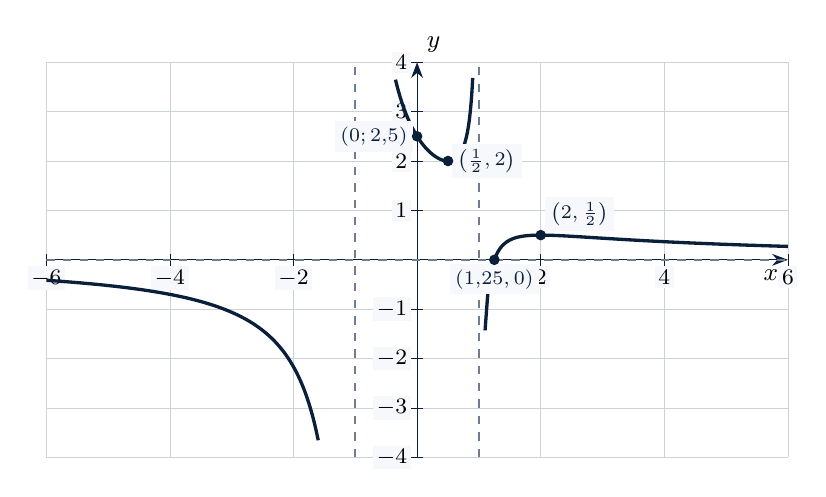
\begin{tikzpicture}
\begin{axis}[
  width=11.0cm, height=6.6cm,
  axis x line=middle, axis y line=middle,
  axis line style={NebulaNavy,-{Stealth[length=2mm]}},
  enlarge x limits=false, enlarge y limits=false,
  xmin=-6, xmax=6, ymin=-4, ymax=4,
  xlabel={$x$}, ylabel={$y$},
  xlabel style={at={(axis description cs:1.0,0.500)},anchor=north east,font=\small},
  ylabel style={at={(axis description cs:0.500,1.0)},anchor=south west,font=\small},
  xtick distance=2, ytick distance=1,
  scaled ticks=false,
  xticklabel style={font=\footnotesize,anchor=north,fill=NebulaBG,inner sep=1.3pt,/pgf/number format/1000 sep={\,}},
  yticklabel style={font=\footnotesize,anchor=east,fill=NebulaBG,inner sep=1.3pt,/pgf/number format/1000 sep={\,}},
  grid=both, grid style={NebulaMuted!35,very thin}, tick style={NebulaNavy}, clip=true,
]
\addplot[NebulaMuted,dashed,thick] coordinates {(-1,-4) (-1,4)};
\addplot[NebulaMuted,dashed,thick] coordinates {(1,-4) (1,4)};
\addplot[NebulaMuted,dashed,thick] coordinates {(-6,0) (6,0)};
\addplot[NebulaNavy,very thick,smooth,samples=100,domain=-6:-1.6] {(4*x-5)/(2*(x^2-1))};
\addplot[NebulaNavy,very thick,smooth,samples=100,domain=-0.35:0.9] {(4*x-5)/(2*(x^2-1))};
\addplot[NebulaNavy,very thick,smooth,samples=100,domain=1.1:6] {(4*x-5)/(2*(x^2-1))};
\addplot[only marks,mark=*,NebulaNavy,mark size=1.7pt] coordinates {(0.5,2)};
\node[font=\scriptsize,NebulaNavy,anchor=west,fill=NebulaBG,inner sep=2pt,outer sep=1.5pt] at (axis cs:0.5,2) {$\left(\tfrac12,2\right)$};
\addplot[only marks,mark=*,NebulaNavy,mark size=1.7pt] coordinates {(2,0.5)};
\node[font=\scriptsize,NebulaNavy,anchor=south west,fill=NebulaBG,inner sep=2pt,outer sep=1.5pt] at (axis cs:2,0.5) {$\left(2,\tfrac12\right)$};
\addplot[only marks,mark=*,NebulaNavy,mark size=1.7pt] coordinates {(0,2.5)};
\node[font=\scriptsize,NebulaNavy,anchor=east,fill=NebulaBG,inner sep=2pt,outer sep=1.5pt] at (axis cs:0,2.5) {$(0;2{,}5)$};
\addplot[only marks,mark=*,NebulaNavy,mark size=1.7pt] coordinates {(1.25,0)};
\node[font=\scriptsize,NebulaNavy,anchor=north,fill=NebulaBG,inner sep=2pt,outer sep=1.5pt] at (axis cs:1.25,0) {$(1{,}25,0)$};
\end{axis}
\end{tikzpicture}
\end{document}
